\section{Modeling of Vapor Intrusion}


\begin{frame}
  \frametitle{Developing a VI Model}
\begin{columns}[T]
    \begin{column}{0.5\textwidth}
      \begin{figure}
        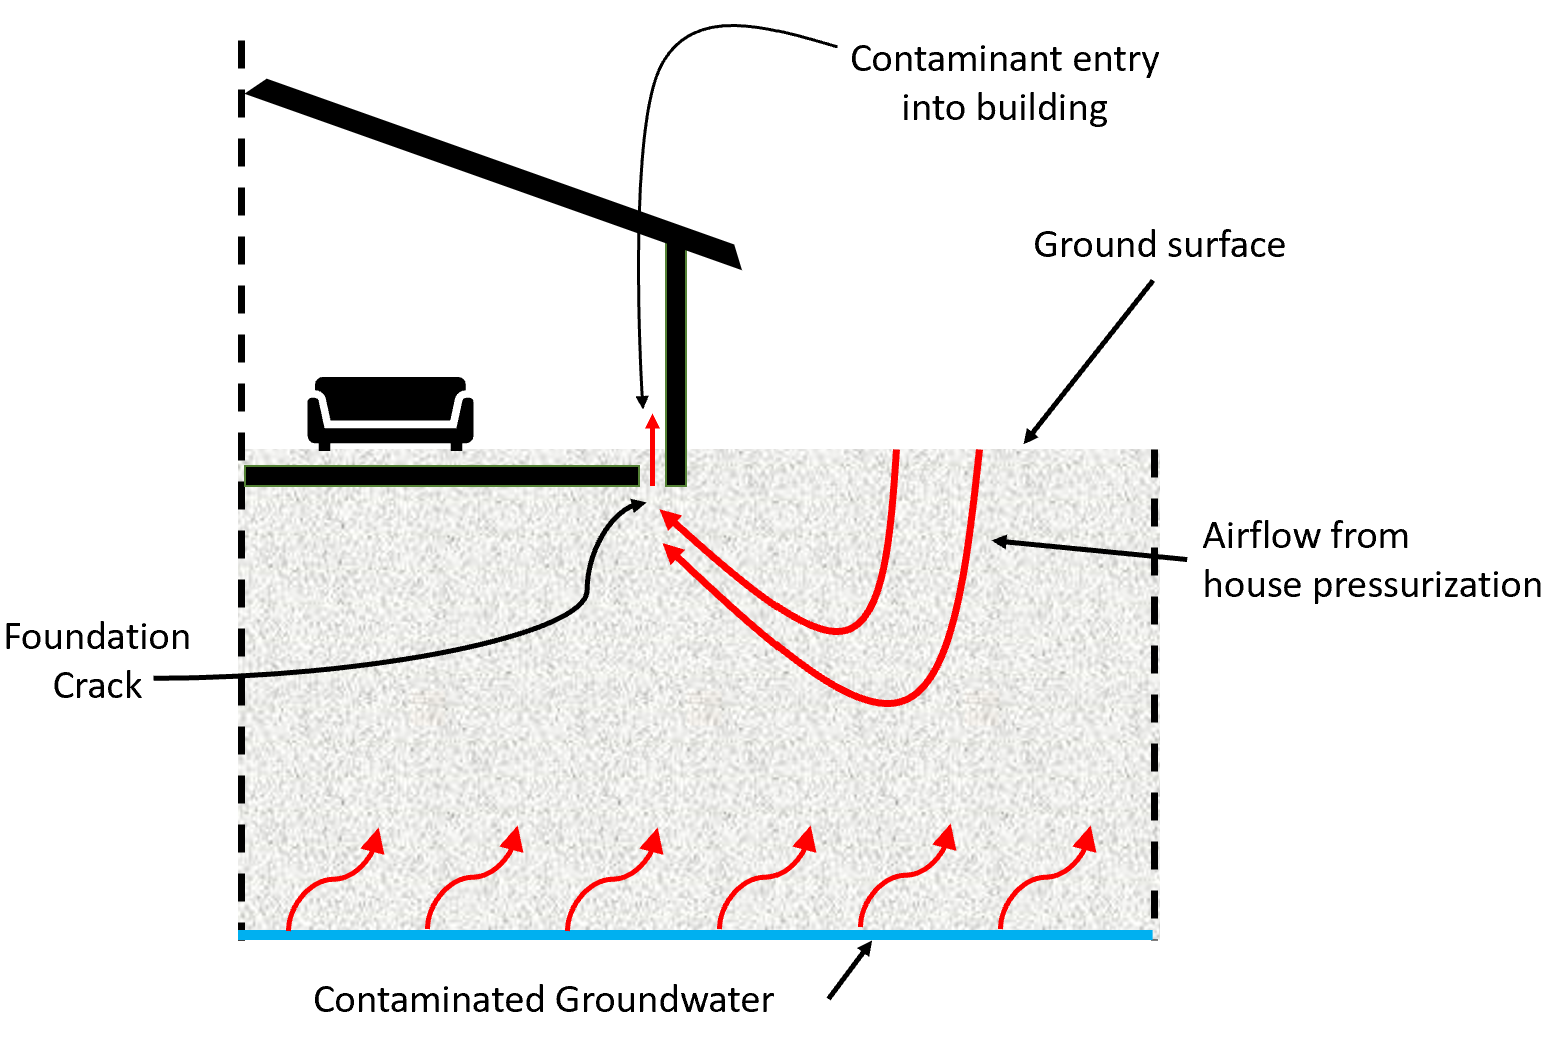
\includegraphics[width=\textwidth]{model_cartoon.png}
      \end{figure}
    \end{column}
    \begin{column}{0.5\textwidth}
      \begin{block}{Physics}
        \begin{itemize}
          \item Indoor environment (CSTR)
          \begin{itemize}
            \item Contaminant entry through foundation crack
            \item Expulsion via air exchange rate
            \item (Indoor sources/sorption possible)
          \end{itemize}
          \item Airflow (Darcy's Law)
          \item Advection-diffusion in soil
          \begin{itemize}
            \item Water/vapor/(sorbed) phases
            \item Biodegradation
          \end{itemize}
          \item Soil moisture content
          \begin{itemize}
            \item Effective permeability
            \item Effective diffusivity
          \end{itemize}
        \end{itemize}
      \end{block}
    \end{column}
  \end{columns}
\end{frame}

\begin{frame}
  \frametitle{Modeling in VI}
\begin{columns}[T]
  \begin{column}{0.5\textwidth}
    \begin{block}{Analytic models}
      \begin{itemize}
        \item Constrained by CSM
        \item 1D (some 2D)
        \item Sacrifice physics to be solvable
        \item Usually steady-state only
      \end{itemize}
    \end{block}
  \end{column}
  \begin{column}{0.5\textwidth}
    \begin{block}{Numerical models}
      \begin{itemize}
        \item Finite-element method
        \item 3D
        \item Adapt/evolve CSM
        \item Resolve all physics
        \item Time-dependent supported
      \end{itemize}
    \end{block}
  \end{column}
\end{columns}


\end{frame}
